\section{Experimental Results}

The proposed MACE algorithm\footnote{Available at https://github.com/Alaya-in-Matrix/MACE} was tested using eight benchmark functions and two
real-world analog circuits. Four state-of-the-art parallel Bayesian optimization
methods were compared, including the BLCB
algorithm~\cite{desautels2014parallelizing}, the local penalization method with
EI acquisition function (EI-LP)~\cite{gonzalez2016batch}, the qEI and qKG
methods~\cite{qEI,wu2016parallel}. \footnote{We implemented the BLCB algorithm as
the available open source implementations only allow discrete input. For the
EI-LP method, the code is downloaded from
https://github.com/SheffieldML/GPyOpt. The code for qEI and qKG is downloaded
from https://github.com/wujian16/Cornell-MOE.}

For the MACE, BLCB, and EI-LP method, the ARD squared-exponential kernel is
used and the GP models are fitted by maximum likelihood estimations (MLE); for
the qKG and qEI methods, the ARD Matern52 kernels are used, and the GP
hyperparameters are integrated via MCMC sampling. The Matern52 kernel and MCMC
integration are the default strategies of the qKG and qEI implementations and
it is unclear in the documentation about how to change the GP settings.


\subsection{Benchmark Problems}

We tested the MACE algorithm and other parallel BO methods using eight commonly used benchmark
functions, as summarized in Table~\ref{tab:summaryanalygical}.

\begin{table}[!htb]
    \centering
    \caption{Summary of the analytical benchmark functions}
    \label{tab:summaryanalygical}
    \begin{tabular}{llllllll}
        \toprule
         Function           & Dimension        & Search domain             \\ \midrule
         Branin             & 2                & $[-5,  10]\times[0, 15]$  \\
         Alpine1            & 5                & $[-10, 10]^5$             \\
         Hartmann6          & 6                & $[0,   1]^6$              \\
         Eggholder          & 2                & $[-512, 512]^2$           \\
         Ackley2            & 2                & $[-32, 32]^2$             \\
         Ackley10           & 10               & $[-32, 32]^{10}$          \\
         Rosenbrock2        & 2                & $[-5,  10]^2$             \\
         Rosenbrock10       & 10               & $[-20, 20]^{10}$          \\
        \bottomrule
    \end{tabular}
\end{table}


For all functions except the two 10D functions, we set the number of initial
random sampling to $N_{init} = 20$ and the number of iterations to $N_{iter} =
45$. Batch size is set to $B = 4$, the total number of function evaluations is
$N_{init} + B \times N_{iter}$. For the 10D Ackley and 10D Rosenbrock functions, we set
$N_{init} = 100$ and $N_{iter} = 175$. The experiments were repeated ten
times to average the random fluctuations.

We also ran the MACE algorithm in sequential mode and compared with the EI and LCB
acquisition functions. The sequential EI and LCB based Bayesian optimization
are implemented by setting the batch size $B = 1$ for EI-LP and BLCB
respectively.


The mean convergence plots of the tested algorithms on the benchmark functions
are given in Figure~\ref{fig:CovPlotBenchmark}, the statistics of the final
regrets are listed in Table~\ref{tab:result_analytical}. As can be seen in
Figure~\ref{fig:CovPlotBenchmark} and Table~\ref{tab:result_analytical}, when
running in sequential mode, the MACE algorithm is competitive with the LCB and
EI acquisition functions. The sequential MACE (MACE-1) algorithm gave better
performances than the sequential EI (EI-1) and sequential LCB (LCB-1)
algorithms in the Eggholder, Branin, Hartmann6, Ackley10, and Rosenbrock10
functions. Also, the parallel MACE (MACE-4) gave the best performances among
all the tested algorithms for six out of the eight benchmark functions, and has
shown dramatic speedup compared to the sequential MACE. We also performed
additional experiments with varied batch sizes, the detail of those
experimental results can be seen in the supplementary materials.

\begin{table*}[!htb]
    \centering
    \caption{Statistics of the regrets of the benchmark functions}
    \label{tab:result_analytical}
    \begin{tabular}{lllllllllll}
        \toprule
                & Eggholder                &  Branin              &  Alpine1              & Hartmann6                   \\ \midrule
        MACE-1  & 87.65$\pm$75.83          &  1.05e-5$\pm$1.31e-5          & 2.66305$\pm$1.05844            & 0.0646869$\pm$0.0621189 \\
        LCB-1   & 153.9$\pm$112.8          &  6.86e-5$\pm$1.13e-4          & 5.66812$\pm$1.76973            & 0.125565$\pm$0.122684   \\
        EI-1    & 172.8$\pm$132.2          &  1.62e-2$\pm$1.63e-2          & 2.46061$\pm$1.56079            & 0.110561$\pm$0.146809   \\
        MACE-4  & 46.38$\pm$40.89          &  \textbf{4.62e-6$\pm$6.64e-6} & \textbf{0.903805$\pm$0.835209} & \textbf{0.0275738$\pm$0.052254}  \\
        BLCB-4  & 56.86$\pm$35.91          &  4.32e-5$\pm$6.33e-5          & 1.8843$\pm$0.938873            & 0.06447$\pm$0.0621176   \\
        EI-LP-4 & \textbf{44.68$\pm$56.45} &  2.11e-2$\pm$1.84e-2          & 1.0059$\pm$0.456865            & 0.0540446$\pm$0.0558557 \\
        qKG-4   & 106.4$\pm$67.64          &  2.65e-1$\pm$2.70e-1          & 3.01513$\pm$1.13414            & 0.47134$\pm$0.18939     \\
        qEI-4   & 72.13$\pm$52.08          &  3.29e-4$\pm$1.14e-3          & 2.7074$\pm$1.05145             & 0.186088$\pm$0.116323   \\
        \hline
                & Ackley2                       &  Rosenbrock2               & Ackley10              & Rosenbrock10        \\ \midrule
        MACE-1  & 1.71474$\pm$1.12154           &  0.026173$\pm$0.051189              & 3.1348$\pm$0.447874           & 499.697$\pm$300.899 \\
        LCB-1   & 1.624$\pm$0.926437            &  0.0201124$\pm$0.0205367            & 3.14797$\pm$0.519164          & 517.944$\pm$288.955 \\
        EI-1    & 1.0136$\pm$0.985858           &  13.5508$\pm$9.52734                & 18.8006$\pm$0.652136          & 1367.08$\pm$637.507 \\
        MACE-4  & 1.07906$\pm$0.886466          &  \textbf{0.00095416$\pm$0.00093729} & \textbf{2.56439$\pm$0.535488} & \textbf{158.116$\pm$50.0024} \\
        BLCB-4  & 1.40051$\pm$1.02849           &  0.00191986$\pm$0.00180895          & 3.27543$\pm$0.735501          & 406.819$\pm$127.351 \\
        EI-LP-4 & \textbf{0.284265$\pm$0.24634} &  2.73645$\pm$2.05923                & 18.2682$\pm$0.608564          & 721.351$\pm$327.365 \\
        qKG-4   & 5.59394$\pm$1.80595           &  5.03976$\pm$3.72014                & 18.197$\pm$0.764103           & 705.112$\pm$412.762 \\
        qEI-4   & 2.87373$\pm$1.02405           &  10.1881$\pm$15.0432                & 18.3686$\pm$0.501869          & 655.208$\pm$340.954 \\
        \bottomrule
    \end{tabular}
\end{table*}


% when running with batch size $B = 4$, the
% MACE algorithm gives the best performance for six out of the eight benchmarks.
% For the 2D Ackley function, EI-LP is the best algorithm, while for the
% Eggholder function, the MACE, BLCB, and EI-LP have quite similar performance.
% Compare the batch MACE and the sequential MACE, the speedup is also dramatic.

\subsection{Operational Amplifier}

%TODO: Introduce the importance of OpAmp and PA

The operational amplifier~\cite{wang2014enabling} shown in
Figure~\ref{fig:schDAC2014} is used to test Bayesian optimization algorithms. The circuit is designed
using the 180nm process. It has 10 design parameters, including the lengths
and widths of transistors, the resistance of the resistors and the capacitance of the
capacitors. The circuit is simulated using the commercial HSPICE circuit simulator.

\begin{figure}[!htb]
    \begin{center}
        \centerline{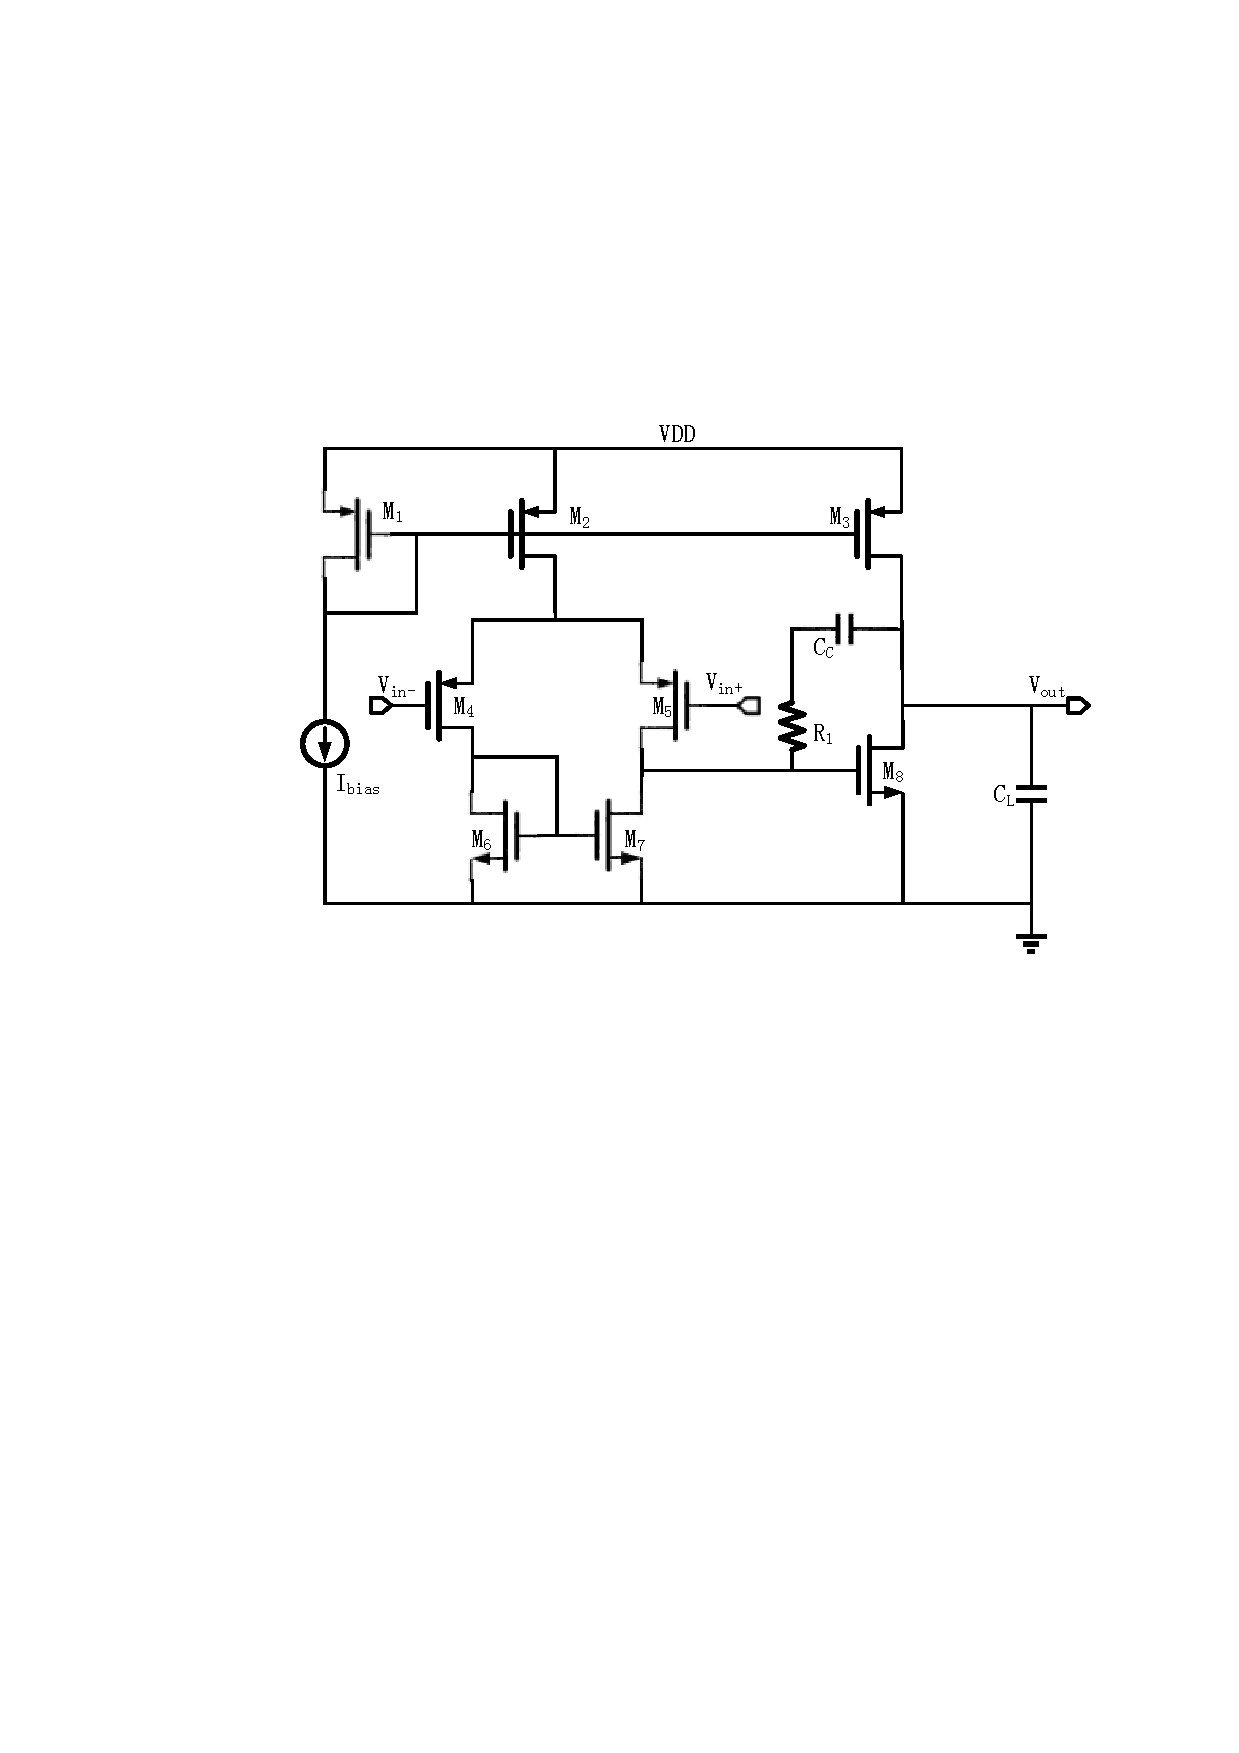
\includegraphics[width=\columnwidth]{./img/sopam.pdf}}
        \caption{Schematic of the operational amplifier}
        \label{fig:schDAC2014}
    \end{center}
    \vskip -0.2in
\end{figure}

We want to maximize the gain, unit gain frequency (UGF) and the phase margin (PM) for this amplifier. The Figure of Merit $FOM$ is constructed as
$$
\mathit{FOM} = -1.2 \times \mathit{gain} - 10 \times \mathit{UGF} - 1.6 \times \mathit{PM}.
$$

For this circuit, we compared the MACE algorithm with the BLCB and EI-LP
algorithms. The qKG and qEI are not compared as the computation of qEI and qKG
acquisition functions become very slow for the ten-dimensional functions.

\begin{figure}[!htb]
\vskip 0.2in
\begin{center}
\centerline{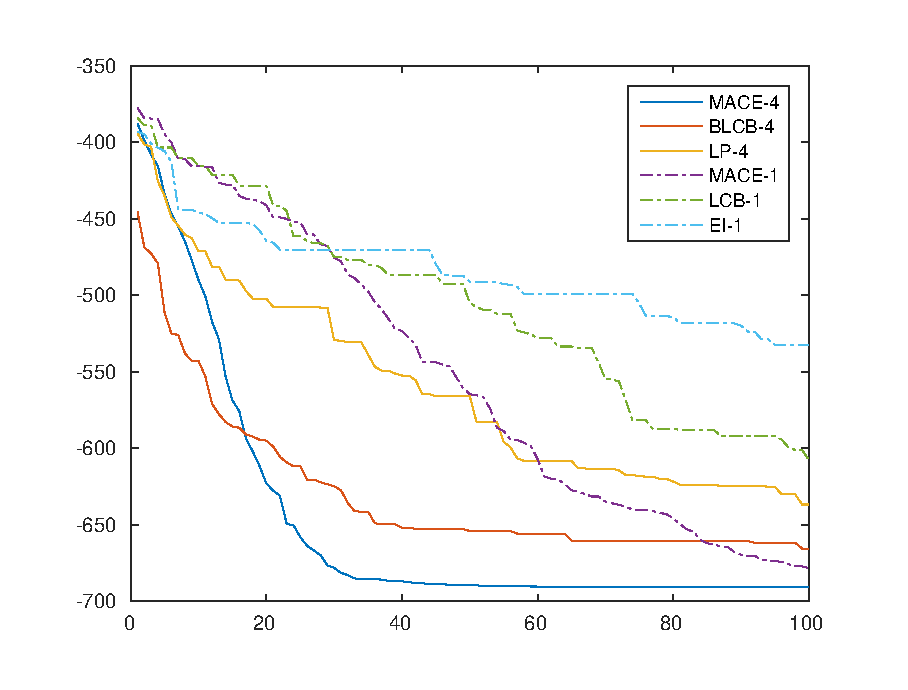
\includegraphics[width=\columnwidth]{./img/mean_DAC2014.eps}}
\caption{Optimization results of the operational amplifier}
\label{fig:resDAC2014}
\end{center}
\vskip -0.2in
\end{figure}


We run the algorithms in sequential mode and batch mode. For the batch mode,
the batch size is set to $B = 4$. The number of initial random sampling is set to
$N_{init} = 100$, and the number of iterations is set to $N_{iter} = 100$.


\begin{table}[!htb]
    \centering
    \caption{Optimization results of the operational amplifier}
    \label{tab:result_opamp}
    \begin{tabular}{llll}
        \toprule
        Algorithm & Results     \\ \midrule
        MACE-1    & -678.174$\pm$21.7445 \\
        LCB-1     & -607.583$\pm$51.9786 \\
        EI-1      & -532.555$\pm$66.942  \\
        MACE-4    & \textbf{-690.3$\pm$0.104963}  \\
        BLCB-4    & -665.442$\pm$23.066  \\
        EI-LP-4   & -636.675$\pm$35.7359 \\
        \bottomrule
    \end{tabular}
\end{table}


The mean convergence plot for the sequential and batch runs are given in
Figure~\ref{fig:resDAC2014}. The mean and standard deviation of the final
optimized FOM values are listed in Table~\ref{tab:result_opamp}. As can be
seen, on average, the batch MACE algorithm had the fastest convergence rate
compared with the sequential MACE algorithm and other parallel algorithms. It
should also be noted that the final optimized FOM values given by MACE-4 have
very small deviation (0.105) compared with other algorithms.

% The mean convergence plot for the sequential and batch runs are shown in
% Figure~\ref{fig:resDAC2014}. As can be seen, the MACE algorithm gave better
% solution compared with other algorithms, the sequential MACE algorithm found
% better solution than BLCB and EI-LP with batch size $B = 4$, which showed that
% the multi-objective acquisition ensemble is more robust than relying on single
% acquisition function; compared with the sequential MACE algorithm, the MACE
% algorithm with batch size $B = 4$ showed considerable speedup.


\begin{figure}[!htb]
    \begin{center}
        \centerline{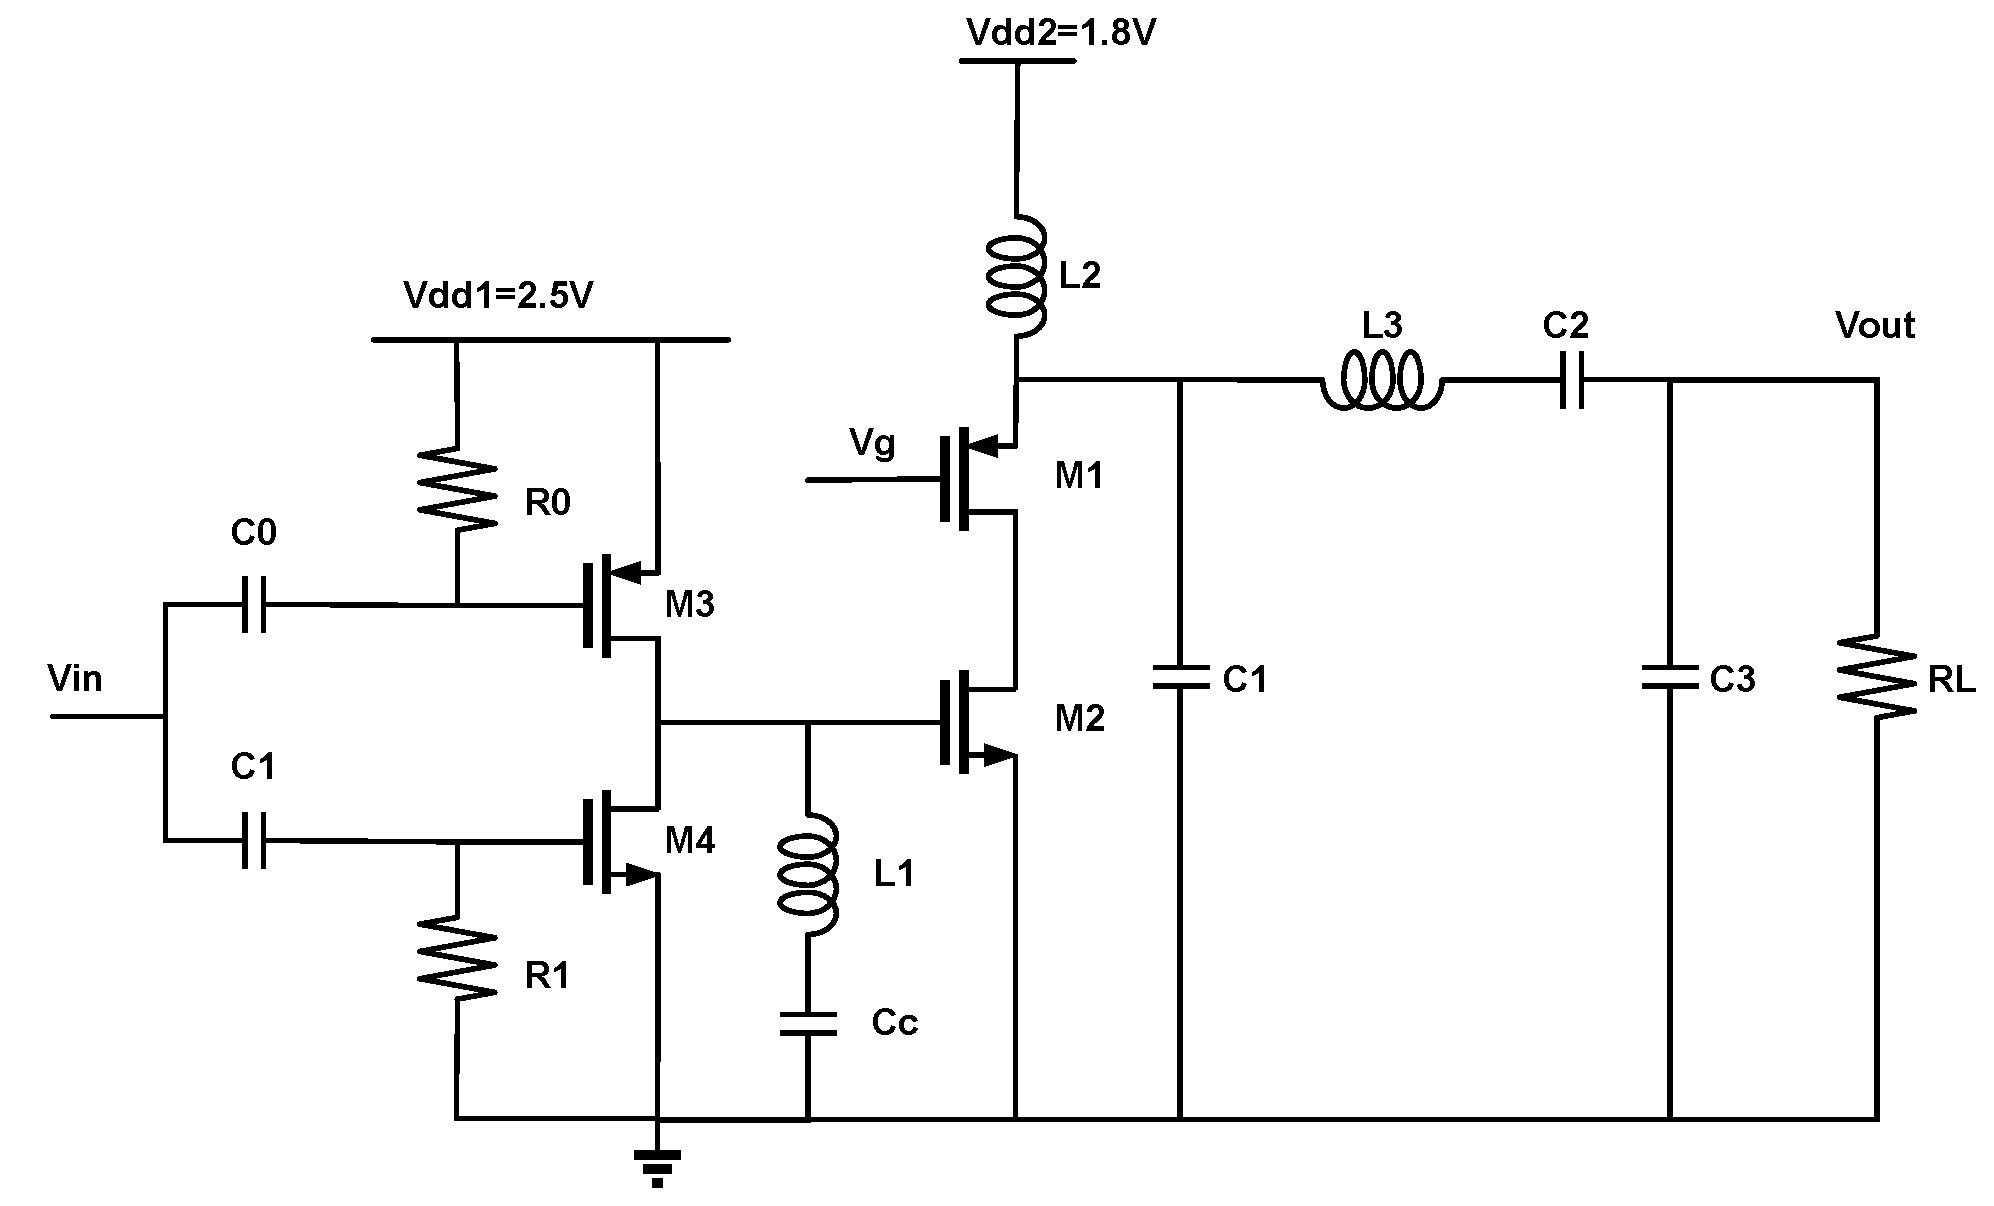
\includegraphics[width=\columnwidth]{./img/classE.eps}}
        \caption{Schematic of the power amplifier}
        \label{fig:schPA}
    \end{center}
    \vskip -0.15in
\end{figure}

\subsection{Class-E Power Amplifier}


The class-E power amplifier shown in Figure~\ref{fig:schPA} is used to test Bayesian optimization algorithms. The
circuit is designed using the 180nm process with 12 design parameters, the
circuit is simulated by the commercial HSPICE circuit simulator to get its performances.



For this power amplifier, we aim to maximize the power added efficiency (PAE) and the output power (Pout), the Figure of Merit $FOM$ is constructed as
$$
\mathit{FOM} = -3 \times \mathit{PAE} - \mathit{Pout}.
$$

The MACE, BLCB, and EI-LP algorithms were tested in both sequential and batch
modes. The number of initial sampling is $N_{init} = 100$. The number of
iterations is $N_{iter} = 100$. The batch size is set to $B = 4$. The total
number of HSPICE simulations is 500 for each batch run and 200 for each
sequential run.

\begin{figure}[!htb]
    \begin{center}
        \centerline{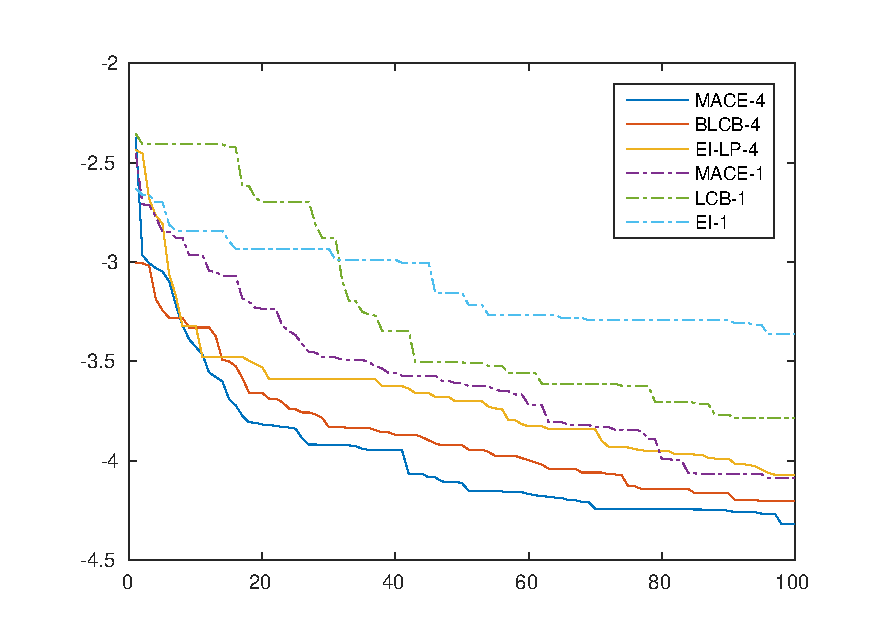
\includegraphics[width=\columnwidth]{./img/ClassE_mean.eps}}
        \caption{Optimization results of the class-E power amplifier}
        \label{fig:resClassE}
    \end{center}
    \vskip -0.2in
\end{figure}


The optimization results of the class-E power amplifier are given in
Figure~\ref{fig:resClassE} and Table~\ref{tab:result_PA}. We can see that the
MACE outperformed the BLCB and EI-LP in both sequential and batch mode. For the
batch runs, the MACE converges fastest among the three algorithms, while the
sequential MACE (MACE-1) has comparable performance as the batch EI-LP
(EI-LP-4) method.

\begin{table}[!htb]
    \centering
    \caption{Optimization results of the power amplifier}
    \vskip 0.15in
    \label{tab:result_PA}
    \begin{tabular}{llll}
        \toprule
        Algorithm & Results               \\ \midrule
        MACE-1    & -4.08608$\pm$0.296647 \\
        LCB-1     & -3.78533$\pm$0.335532 \\
        EI-1      & -3.36407$\pm$0.307489 \\
        MACE-4    & \textbf{-4.31762$\pm$0.347026} \\
        BLCB-4    & -4.20266$\pm$0.211102 \\
        EI-LP-4   & -4.07233$\pm$0.244436 \\
        \bottomrule
    \end{tabular}
    \vskip -0.1in
\end{table}
